
Regarding the models, we can classify each model trained by its main idea behind their design:
\begin{itemize}
	\item Simple \gls{cnn}. Due to its simplicity compared to the other architectures, its primary purpose was to determine the level of challenge posed by the dataset.
	\item Residual neural networks. Inspired by \cite{Meraner2020}, it has been developed residual blocks to fit in \gls{cnn} architectures to check the behaviour of the input data and the possible lack of \gls{sar} data.
	\item Autoencoders not only reduces the dimensions of the input data but also it has a new kind of layers called \textit{Convolutional Transposed} layers. This models were designed to know how dimensionality reduction affects to the data.
	\item \gls{vae}. While traditional autoencoders might not fully capture the diverse nuances of the data, contrasting them with likelihood-based models can provide valuable insights into their strengths and limitations.
	\item \gls{gan} have the potential to outperform standard \gls{cnn}s, primarily due to the integration of the discriminator component. The primary focus here will be on preventing mode collapse and ensuring the stability of both the generator and discriminator networks within the GAN architecture.
	\item Finally, a compromising \gls{ddm}s will be explained.
\end{itemize}
\subsubsection{Convolutional Neural Networks}
The training of the simple \gls{cnn} was the initial step in assessing the dataset's complexity. This basic CNN architecture consisted of eight convolutional layers, each followed by a batch normalization layer and the \gls{relu} activation function.
\begin{figure}[H]
	\centering
	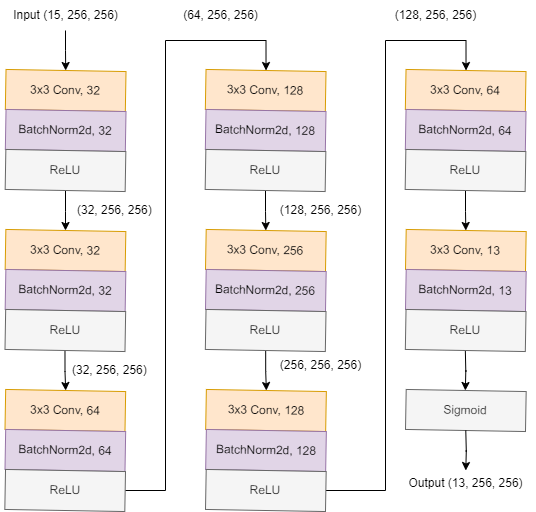
\includegraphics[width=8cm]{imgs/models/models/cnn/CNN.png}
	\caption{Carla model}
	\label{fig:models-carla-loss}
\end{figure}
The purpose of this straightforward \gls{cnn}, called \texttt{Carla}, was to provide a baseline understanding of how challenging it was to learn from the dataset with only \texttt{SEN12MS-CR}. The model has been trained using \gls{mse} loss and with a max-min scaling. By analyzing the performance, we could gauge the inherent complexity of the data and make informed decisions about whether more advanced architectures were necessary. By training this model, it has been demonstrated that small models cannot adequately address the complexity of this problem. This topic will be further discussed in the experiments and results section.
\\
\\
To push forward with our study in generative models and building on the work of \cite{Meraner2020}, it has been developed a model which uses similarly residual blocks of stride 1 to capture the behaviour of \gls{sar} data, as it shows the Figure \ref{fig:residual-block-regina2}.
\begin{figure}[H]
	\centering
	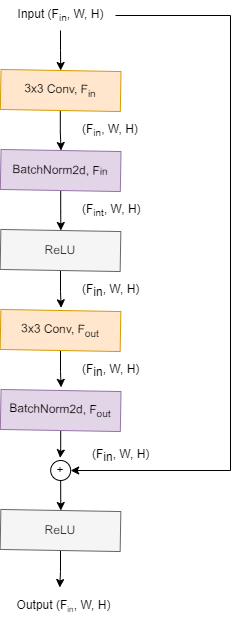
\includegraphics[width=4cm]{imgs/models/models/cnn/ResBlock.png}
	\caption{Residual block from \texttt{Regina}}
	\label{fig:residual-block-regina2}
\end{figure}
What significantly differs between the current model and the inspired model is the number of parameters, which has been reduced to 50\% of the referenced model. Firstly, to reduce parameter dimensionality and prevent gradient-related issues, the number of channels was systematically reduced. While \cite{Meraner2020} always uses 256 filters in each convolution, the filters of the convolutional layers in \texttt{Regina} are added incrementally and then, decrementally. Moreover, the number of blocks was decreased from 16 to 10. To compensate this, for this omission and enhance the model's performance, a sigmoid function was introduced in the final layer to constrain the pixel values within a specific range. 
\begin{figure}[H]
	\centering
	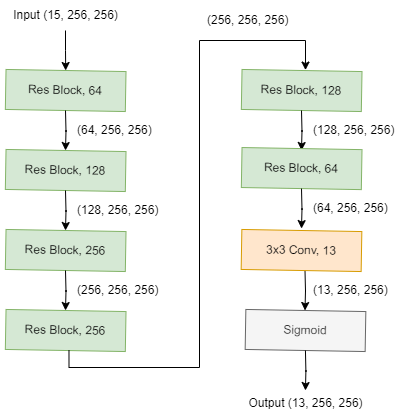
\includegraphics[width=8cm]{imgs/models/models/cnn/Regina.png}
	\caption{Regina architecture }
	\label{fig:residual-block-regina}
\end{figure}
Since the use of \gls{sar} data has also been a prominent topic in the state of the art and to assess whether the inclusion of augmented data enhances the model's performance, multiple training sessions of \texttt{Regina} were conducted, comparing sessions with and without augmented data.

\subsubsection{Autoencoders}
After creating residual models with skip connections, the introduction of autoencoders was proposed to explore how their training and results compared to other models. Unlike the previous models designed, these autoencoders incorporated the use of transposed convolutional layers, which means they generated a kernel based on an input value, as opposed to assigning a value based on a kernel.
\begin{figure}[H]
	\centering
	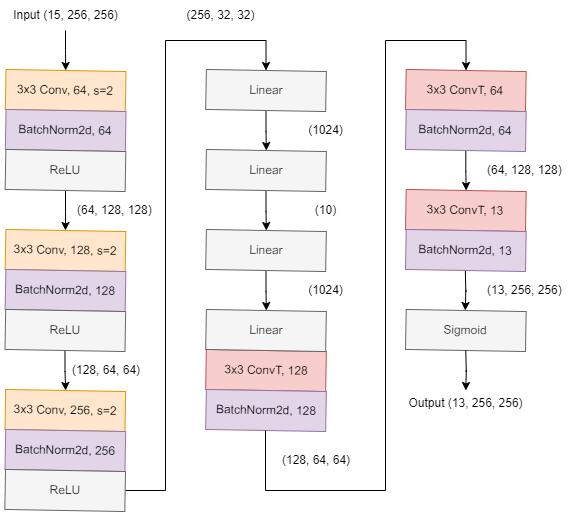
\includegraphics[width=8cm]{imgs/models/models/cnn/Anna.png}
	\caption{Anna architecture }
	\label{fig:residual-anna}
\end{figure}
The initial model, named \texttt{Anna}, was developed to assess the capabilities of de-convolutions for dimensionality reduction. This reduction, which was carried out by striding the convolutions, was also pursued with the aim of exploring the data distribution within a latent space. Similarly, \texttt{Veronica} was created by solely modifying the linear layers in the middle with GlobalAveragePool layers, enabling the determination of the output.
\\
\\The reason behind introducing these transposed convolutional layers at this stage of development was straightforward. The use of deconvolutions allows upsampling and creating new filters at the same time, without involving a new use in memory.
\\
\\
Although the residual blocks in the models had a higher level of complexity and there is no transposed residual convolutional block, when dealing with images having spatial dimensions of \texttt{256x256}, employing autoencoders for dimensionality reduction, latent space exploration, and unsupervised classification might not yield satisfactory results due to a suboptimal model design that results in significant loss during reconstruction. In this sense, the concept of incorporating skip connections was conceived to retain more information in the model.
\begin{figure}[H]
	\centering
	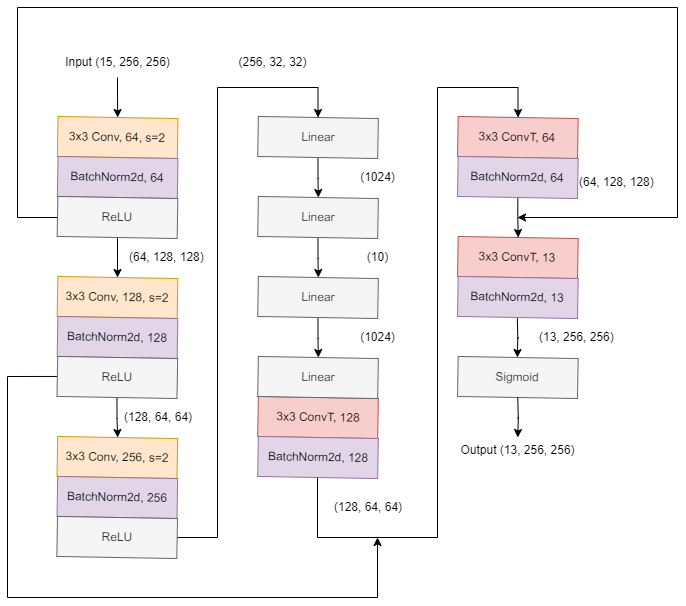
\includegraphics[width=8cm]{imgs/models/models/cnn/AnnaSkip.png}
	\caption{AnnaSkip architecture}
	\label{fig:residual-anna-skip}
\end{figure}
Although it will be shown an improvement with the introduction of skip connections, it still fell short of comparing favorably with other models. Thus, it became apparent that the issue might be rooted in the dimensionality reduction process. To address this limitation, more flexible models were considered, such as the \texttt{U-Net} architecture, where the dimension was not restricted to a one-dimensional vector but comprised different filters with reduced spatial dimensions. This led to the creation of the \texttt{Ausias} model, which, while not converting the image into a 1D vector to analyze its characteristics, yielded better performance metrics.
\subsubsection{Generative Adversarial Networks}
\gls{gan}s have been a majority of the work entailed during the research of cloud removal. It is notable that adversarial training have been a significant popular focus of our research in cloud removal. So, therefore, it's worth emphasizing that the use of adversarial training has been pivotal in our approach.
\\
\\
Although it seems obvious, the most difficult part of training a \gls{gan} is the instability of the training loop, since two neural networks are trying to outdo each other. Finding the right balance between the two networks and achieving convergence is challenging.
\\
\\
Hence, instead of contemplating an architecture where the generative model might struggle to comprehend the dataset, the approach was to use an architecture that demonstrated effectiveness with the existing dataset, which is \texttt{Regina}. Subsequently, an exhaustive research have been pursued for getting the most suitable discriminative models. This involved adding and removing layers, fine-tuning parameters of the optimizers and implementing strategies, which will be elaborated upon below. Estimating the architecture was straightforward, since it is recommendable to start using the same amount of parameter of the generative network. Also, it is a good practice to use LeakyReLU instead of \gls{relu} in order to make the discriminator less smart than the generator. In a standard \gls{relu} function, the output is zero for any input less than or equal to zero and linear (equal to the input) for positive values. LeakyReLU introduces a small, non-zero gradient for negative input values, instead of being completely zero. 

\subsubsection{Denoising Diffusion Models}
Finally, the last section involves discussing diffusion models. Given a lack of domain expertise and uncertainty regarding how this dataset might respond to diffusion models, an effort was made to find a library that would simplify the design process. While it's true that \texttt{Regina} could have been employed as a model, since the only requirement is to use the same spatial dimensions. However, it was deemed unsuitable for this purpose when trained as a denoising model due to perceived limitations in its complexity. Instead, the chosen model was a variant of the UNet with residual downsampling blocks. At each downsampling step, the model incorporates attention mechanisms similar to how \gls{vit} would employ the Scale Dot Product Attention in its attention heads.
\\
\\
The inclusion of spatial self-attention in the downsampling block allows the model to capture long-range dependencies in the image. Traditional convolutional layers have a limited receptive field, meaning they can only capture information from nearby spatial locations. With spatial self-attention, the model can consider information from all parts of the image, making it more powerful and potentially improving its performance on tasks like segmentation.
\\
\\
It's worth noting that attention mechanisms, especially in large models or images, can be computationally intensive. However, their ability to capture long-range dependencies and focus on relevant parts of the input often leads to improved performance in many tasks.
